\vspace{-0.1in}
\section{Introduction}
\label{sec:intro}
\vspace{-0.05in}
Existing datacenters are built using servers, each of which tightly integrates a small amount of the various resources needed for a computing task (CPU, memory, storage). While such server-centric architectures have been the mainstay for decades, recent efforts suggest a forthcoming paradigm shift towards a {\em disaggregated} datacenter (\dis) where each resource type is built as a standalone resource `blade' and a network fabric interconnects these resource blades. Examples of this include Facebook~\cite{fdr}, HP~\cite{hptm}, Intel~\cite{rsa}, SeaMicro~\cite{seamicro} as well as prototypes from the computer architecture community~\cite{firebox, sonuma, ddcHwDesign1}. 

These industrial and academic efforts have been driven largely by hardware architects because CPU, memory and storage technologies exhibit significantly different trends in terms of cost, performance and power scaling~\cite{memristors,nvram,reg-ex-hardware,gpus}. This, in turn, makes it increasingly hard to adopt evolving resource technologies within a server-centric architecture (\eg, the memory-capacity wall making CPU-memory co-location unsustainable~\cite{ddcHwDesign1}). By decoupling these resources, \dis makes it easier for each resource technology to evolve independently, and reduces the time-to-adoption by avoiding the burdensome process of redoing integration and motherboard design. In addition, disaggregation also enables fine-grained and efficient provisioning and scheduling of individual resources across jobs~\cite{hotnets}. 


A key enabling or blocking factor for disaggregation will be the network since disaggregating CPU from memory and disk requires that the inter-resource communication that used to be contained \emph{within} a server must now traverse the network fabric. 
Thus to be able to offer good application-level performance it becomes critical that the network fabric provide low latency communication for this increased load. 
It is perhaps not surprising then that prototypes from the hardware community~\cite{rsa, fdr, hptm, seamicro, firebox, sonuma, ddcHwDesign1} all rely on new high-speed network components -- e.g., silicon photonics or PCIe switches and links, new interconnect fabrics, etc.
The problem however is that these new technologies are still a long way from matching existing commodity solutions with respect to cost efficiency,  manufacturing pipelines, support tools, and so forth. Hence, at first glance, disaggregation would appear to be gated on the widespread availability of new networking technologies. 

But are these new technologies strictly \emph{necessary} for disaggregation? 
Somewhat surprisingly, despite the many efforts towards and benefits of resource disaggregation, there has been little systematic evaluation of the network requirements for disaggregation. 
In this paper, we take a first stab at evaluating the \emph{minimum} (bandwidth and latency) requirements that the network in disaggregated datacenters must provide. We view the minimum requirement for the network is that it allow us to maintain application-level performance close to server-centric architectures; i.e., at minimum, we aim for a network that keeps application performance degradation small while still enabling the aforementioned qualitative benefits of resource disaggregation.

\eat{
{\footnote{\rc{In the longer term one might expect to re-architect existing applications to exploit \dis for better performance (e.g., by leveraging remote memory); in the shorter term, which is our focus, all we can hope for is that the application performance degradation (due to CPU-memory disaggregation) is small while still reaping the aforementioned qualitative benefits of resource disaggregation.}}}, 
}

%The heretofore unexamined questions, which we address here, are (i) just what are these latency and bandwidth requirements, and (ii) are they feasible with today's technologies.
%
\eat{
This paper takes a first step towards addressing these questions. That is, rather than proposing a new network design, this paper systematically explores: (i) the (bandwidth and latency) requirements from the network fabric in resource disaggregated datacenters, and (ii) how well do existing (deployed or proposed) designs meet these requirements. \eat{We also use our findings (summarized below) to critically explore the assumptions and design decisions made in existing disaggregated prototypes and to identify gaps in existing network designs, and discuss how these observations can guide the design of network hardware and network stacks for resource disaggregated datacenters. \rc{$\gets$ Don't like this para much; sounds like a weak first preview of our work}
}
}

We evaluate these minimum network requirements in the context of ten workloads spanning seven popular open-source systems --- Hadoop, Spark, GraphLab, Timely dataflow~\cite{timely-dataflow, timely-dataflow1}, Spark Streaming, memcached~\cite{memcached}, HERD~\cite{herd}, and SparkSQL. 
\eat{off-disk batch processing using Hadoop, in-memory batch processing using Spark, distributed graph processing using GraphLab, highly  optimized graph processing using Timely dataflow~\cite{timely-dataflow, timely-dataflow1}, stream processing using Spark Streaming, point queries with memcached~\cite{memcached} and HERD~\cite{herd}, and an optimized in-memory SQL engine SparkSQL. 
}
As we elaborate on in \S\ref{sec:requirements}, we focus on current applications such as the above because they represent the worst case in terms of the application \emph{degradation} that may result from disaggregation. 


\noindent Our key findings are:
\vspace{-0.5em}
\begin{itemize}[leftmargin=*]
\itemsep0em
	\item Network bandwidth in the range of $40-100$Gbps  is sufficient to maintain application-level performance similar to existing datacenters; this is easily in reach of existing switch and NIC hardware. 
	\eat{
	\rqc{Could we say the impact of 1Tbps links on application-level performance?} \rc{Our analysis suggests this conclusion will hold even in the face of app optimization (), increasing core density (), and data density ()
	}
	}
	%
	\item Network latency in the range of $3-5\mu$s is needed to maintain application-level performance. This is a challenging task. Our analysis suggests that the primary latency bottleneck stems from  network software rather than hardware: we find the latency introduced by the endpoint is roughly $66\%$ of the inter-rack latency and roughly $81\%$ of the intra-rack latency. Thus many of the optimizations being pursued by switch hardware architects~\cite{mellanox} optimize the relatively smaller fraction of the overall latency budget; instead, work on bypassing the kernel for packet processing and NIC integration~\cite{cpu-nic} could significantly impact the feasibility of resource disaggregation.
	%
	\item We show that the above requirements follow from the memory bandwidth demands of applications.
	\item While most efforts focus on disaggregating at the rack scale, our results show that for many applications disaggregation at the datacenter scale is entirely feasible.	%
 	\item Finally, our study shows that transport protocols frequently deployed in today's datacenters (TCP or DCTCP) fail to meet our target requirements for low latency communication with the \dis workloads. However, some recent research proposals~\cite{pfabric, phost} do provide the necessary end-to-end latencies. 
\end{itemize} 

\noindent
Taken together, our study suggests that resource disaggregation need not be gated on the availability of new networking hardware: instead, minimal performance degradation can be achieved with existing network hardware (either commodity, or available shortly).
%and in many cases can be applied across the datacenter, not just within a rack. 
%Our findings are thus in contrast with many industrial or commercial efforts that rely on new network designs and technologies, or focus only on rack-scale disaggregation.

There are two important caveats to this.  First, while we may not need network changes, we will need changes in hosts, for which RDMA and NIC integration (for hardware) and pFabric or pHost (for transport protocols) are promising directions. Second, our point is not that new networking technologies are not worth pursuing but that the adoption of disaggregation \emph{need not be coupled} to the deployment of these new technologies. Instead, early efforts at disaggregation can begin with existing network technologies and the newer technologies can be incorporated as and when it makes sense from a performance, cost, and power standpoint.
%Likewise, re-architect existing applications to exploit \dis for better performance (e.g., by leveraging remote memory) 

Before continuing, we note three limitations of our work. First, our results are based on ten specific workloads spanning seven open-source systems with varying designs; we leave to future work an evaluation of whether our results generalize to other systems and workloads.
%\rc{, but note that even ``new-world''/highly optimized (HERD) systems have perf comparable to other systems we measure}. 
Second, we focus primarily on questions of network design for disaggregation, ignoring many other systems questions (\eg, scheduler designs or software stack) modulo discussion on understanding latency bottlenecks. However, if the latter does turn out to be the more critical bottleneck for disaggregation, one might view our study as exploring whether the network can `get out of the way' (as often advocated~\cite{greenberg-sigcomm15}) even under disaggregation. Finally, our work looks ahead to an overall system that does not yet exist and hence we must make assumptions on certain fronts (e.g., hardware design and organization, data layout, etc.). We make what we believe are sensible choices, state these choices explicitly in \S\ref{sec:summary}, and to whatever extent possible, evaluate the sensitivity of these choices on our results. Nonetheless, our results are dependent on these choices and more experience is needed to confirm their validity.

\begin{figure*}[!h]
\centering 
\subfigure[Current datacenter] {
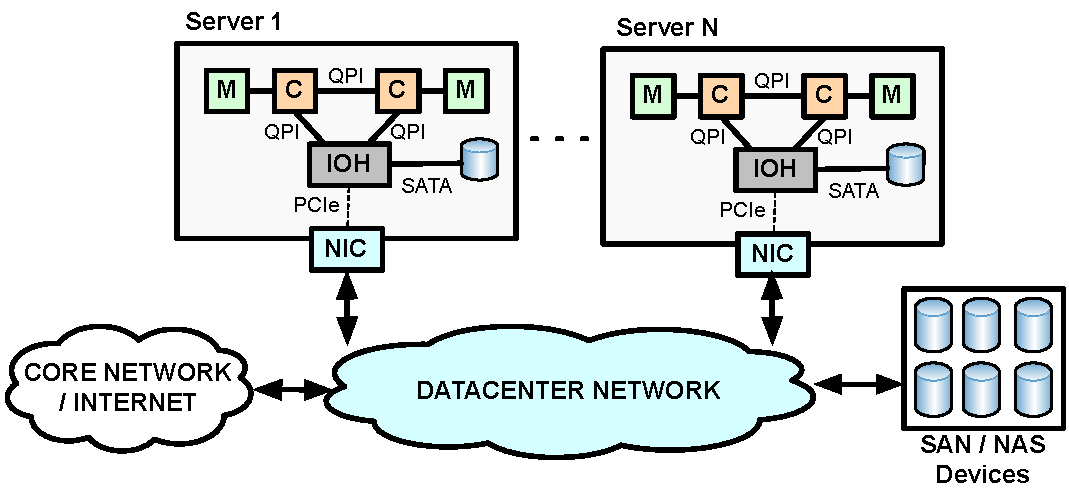
\includegraphics[width=2.6in]{img/DC_before_4.pdf}
\label{subfig:dc_before}
}
%\hfill
\subfigure[Disaggregated datacenter] {
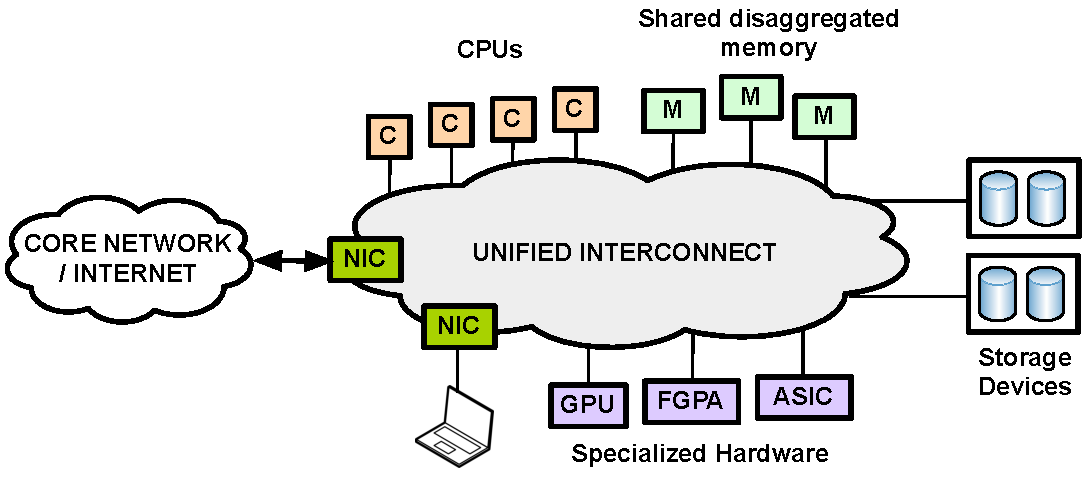
\includegraphics[width=2.6in]{img/DC_after_2.pdf}
\label{subfig:dc_after}
}
\caption{High-level architectural differences between server-centric and resource-disaggregated datacenters.}
\label{fig:dc}
\end{figure*}